\input{../Plantillas-Fomato/Tareas/tarea.tex}
\tcabe{introducción a las probabilidades}{Jhonny Lanzuisi, 1510759}
\cabe{introducción a las probabilidades: segundo parcial}
\begin{document}
	\thispagestyle{plain}
\chapter*{Segundo Parcial}
\subsection*{Ejercicio 1}
\begin{sol}
	Sea $X$ la cantidad de pelotas verdes que aparecen, entonces $X$ es una variable aleatoria binomial (debido a que hay reemplazo) con parámetros $(n=3,p=1/3)$ ---el parámetro $p$ se obtiene de que la probabilidad de sacar una pelota verde es $2/6$---.
	
	Entonces la probabilidad viene dada por
	\begin{equation}
		p(i) = \binom{n}{i}p^i(1-p)^{n-i} \quad i=0,1,2,3
	\end{equation}
	que explícitamente es
	\begin{align*}
		P\{X=0\}  &= \binom{3}{0} \left(\frac 13\right)^0 \left(\frac 23\right)^3 = \frac{8}{27} \approx 0.30 \\
		P\{X=1\}  &= \binom{3}{1} \left(\frac 13\right)^1 \left(\frac 23\right)^2 = \frac{4}{9} \approx 0.44 \\
		P\{X=2\}  &= \binom{3}{2} \left(\frac 13\right)^2 \left(\frac 23\right)^1 = \frac{2}{9} \approx 0.22 \\
		P\{X=3\}  &= \binom{3}{3} \left(\frac 13\right)^3 \left(\frac 23\right)^0 = \frac{1}{9} \approx 0.04. 
	\end{align*}
	Su distribución viene dada por la gráfica:
	\begin{figure}[H]
		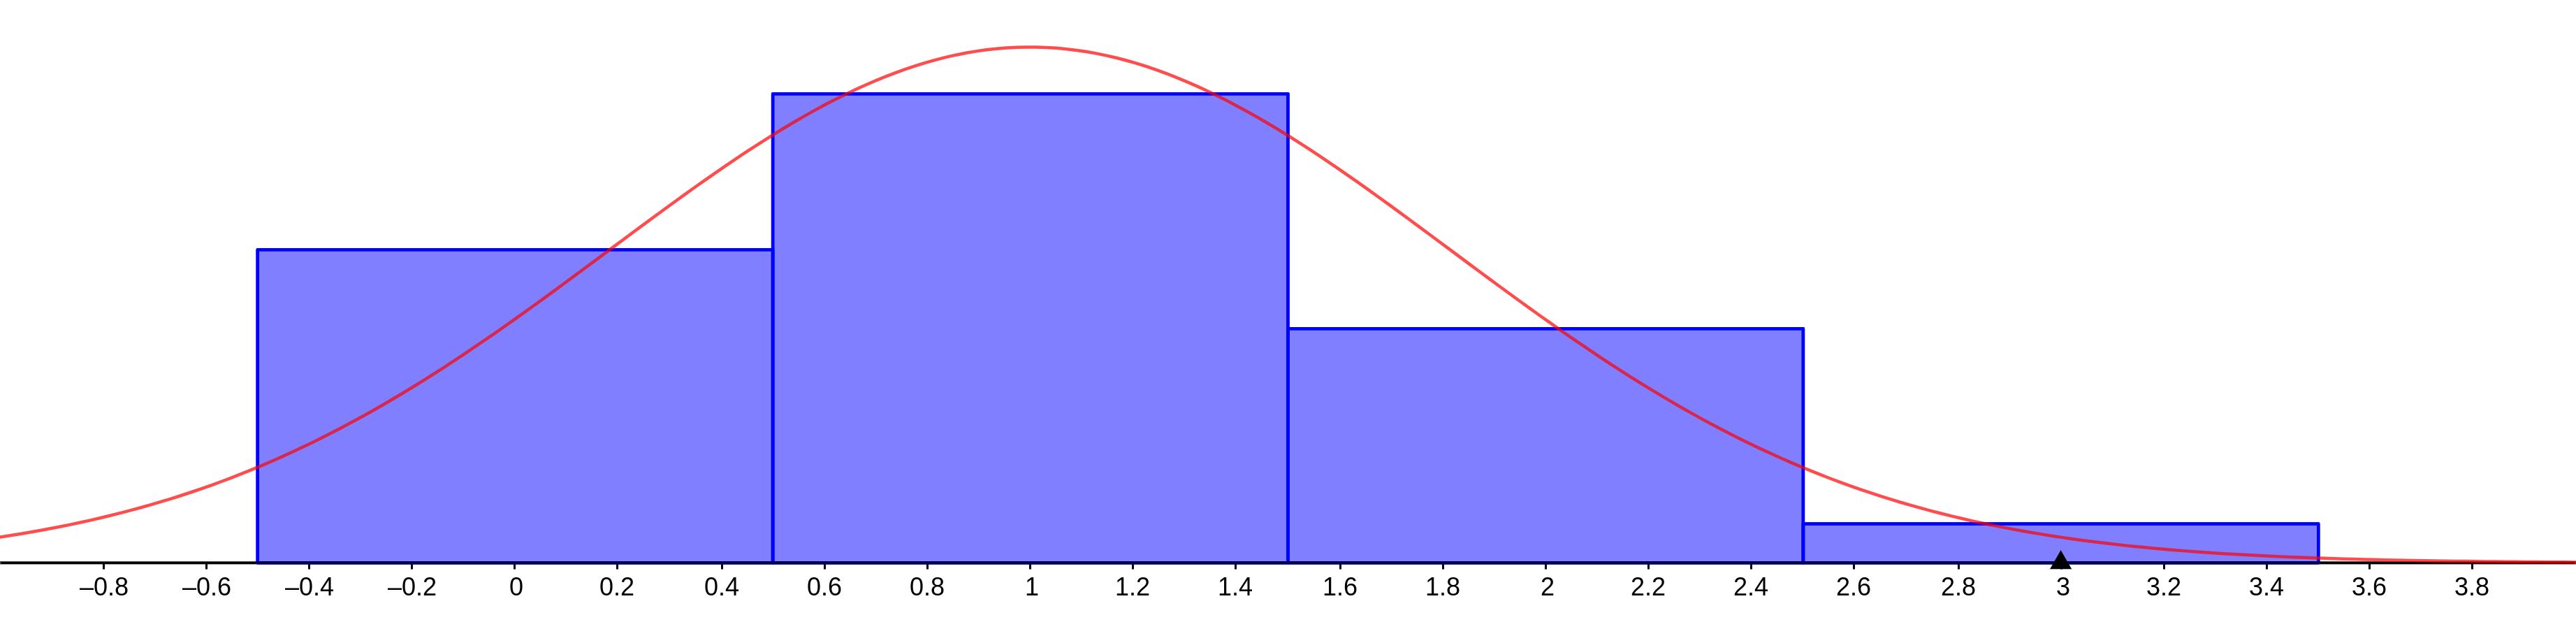
\includegraphics[width=0.6\linewidth]{pics/p1}
		\centering
	\end{figure}
	\noindent Y su distribución acumulada es
	\[ 
	F(b) = \begin{cases}
		  \hspace{1em} 0 \hspace{1.9em} \text{si} \; b<0 \\
		  \hspace{.5em} 0,30 \quad \text{si} \; 0 \leq b < 1\\
		  \hspace{.5em} 0,74 \quad \text{si} \; 1\leq b < 2\\
		  \hspace{.5em} 0,96 \quad \text{si} \; 2\leq b < 3\\
		  \hspace{1em} 1 \hspace{1.9em} \text{si} \; 3\leq b 
		   \end{cases}
	\]

\end{sol}
\subsection*{Ejercicio 2}
	Suponga que 10 aparatos de radar están operando independientemente uno del otro y que la probabilidad
	de que sólo uno de los aparatos detecte un cohete enemigo es de 0.80. ¿Cuál es la probabilidad de que nueve
	aparatos de radar detecten el cohete?

\begin{sol}
	Este problema sigue una distribución binomial, al igual que el anterior, pero con los parametros $n=10$ y $p=0.80$. Sea $X$ la cantidad de aparatos de radar que detectan un cohete, entonces la probabilidad buscada es, por la ecuación $(1)$,
	\[ P\{X=9\} = \binom{10}{9}(0,8)^9(0,2)^1 \approx 0.27. \]
\end{sol}
\subsection*{Ejercicio AKI}
	El promedio de automóviles que entran a la montaña por el túnel es de uno cada dos minutos. Si un
	numero excesivo de autos entra por el túnel en un periodo corto se produce una situación peligrosa. Encuentre la
	probabilidad de que el número de automóviles que entra al túnel durante un periodo de dos minutos exceda a tres.
	¿Parece razonable el uso de Poisson en este problema?

\begin{sol}
	Usaremos la distribución Poisson. Sea $X$ el número de automóviles que entran en el túnel, entonces $X$ sigue una distribución Poisson con parámetro $\lambda=1$. La probabilidad buscada es:
	\[ P\{X>3\} = 1 - P\{X\leq 2\} = 1 -  P\{X=0\} -P\{X=1\}-P\{X=2\}. \]
	Calculando las probabilidades que nos hacen falta, tenemos:
	\begin{align*}
		P\{X=0\} &= e\inv \frac{1^0}{0!} \\
		P\{X=1\} &= e\inv \frac{1^1}{1!} \\
		P\{X=2\} &= e\inv \frac{1^2}{2!} 
	\end{align*}	
	Finalmente, la probabilidad buscada es:
	\[ P\{X>3\} = 1 -  e\inv \frac{1^0}{0!} - e\inv \frac{1^1}{1!} - e\inv \frac{1^2}{2!} \approx 0.08. \]
\end{sol}
\subsection*{Ejercicio 3}
	Unas especificaciones piden que un tipo de termistor soporte entre 9 y 10 mil ohm a 25°C. De 19
	termistores disponibles, se seleccionarán cuatro para usarlos. Sea $X$ el número entre los cuatro que no se apegue
	a las especificaciones. Calcular la distribución de probabilidad de $X$, en forma tabular, si:
	\begin{enumerate}
		\item entre los 19 hay dos que no se apegan a las especificaciones,
		\item entre los 19 hay cuatro que no se apegan a las especificaciones.
	\end{enumerate}

\begin{sol}
	Sea $X$ como en el enunciado. Entonces $X$ sigue una distribución hipergeométrica cuya probabilidad viene dada por
	\begin{equation}
		P\{ X=i \} = \frac{\binom{N_p}{i} \binom{N-N_p}{n-i}}{\binom{N}{n}} \quad i=1,2,\cdots, \min(n,N_p).
	\end{equation}
	Veamos ahora cada parte.
	\begin{enumerate}
		\item Los parámetros que usaremos en este caso son $n=4,N_p=2,N=19,N-N_p=17$. Así obtenemos, por la ecuación $(2)$:
		\begin{align*}
			P\{X=0\} &= \frac{\binom{2}{0} \binom{17}{4}}{\binom{19}{4}} = \frac{2380}{3876} \approx 0.61 \\
			P\{X=1\} &= \frac{\binom{2}{1} \binom{17}{3}}{\binom{19}{4}} = \frac{2(680)}{3876} \approx 0.35 \\
			P\{X=2\} &= \frac{\binom{2}{2} \binom{17}{2}}{\binom{19}{4}} = \frac{136}{3876} \approx 0.04 
		\end{align*}
		\item En este caso, usaremos los parámetros $n=4,N_p=4,N=19,N-N_p=15$. Obtenemos entonces:
		\begin{align*}
		P\{X=0\} &= \frac{\binom{4}{0} \binom{15}{4}}{\binom{19}{4}} = \frac{1365}{3876} \approx 0.35 \\
		P\{X=1\} &= \frac{\binom{4}{1} \binom{15}{3}}{\binom{19}{4}} = \frac{4(455)}{3876} \approx 0.47 \\
		P\{X=2\} &= \frac{\binom{4}{2} \binom{15}{2}}{\binom{19}{4}} = \frac{6(105)}{3876} \approx 0.16 \\
		P\{X=3\} &= \frac{\binom{4}{3} \binom{15}{1}}{\binom{19}{4}} = \frac{4(15)}{3876} \approx 0.02 \\
		P\{X=4\} &= \frac{\binom{4}{4} \binom{15}{0}}{\binom{19}{4}} = \frac{1}{3876} \approx 0 
		\end{align*}
	\end{enumerate}
\end{sol}
\subsection*{Ejercicio 4}
	Se supone que 30\% de los aspirantes para cierto trabajo industrial tiene un entrenamiento avanzado
	en programación. Los aspirantes son entrevistados, uno tras otro, y son seleccionados al azar del conjunto de
	aspirantes. Determine la probabilidad de que se encuentre el primer aspirante con un entrenamiento avanzado en
	programación en la quinta entrevista.

\begin{sol}
	Sea $X$ la variable aleatoria que representa el número de entrevistas para obtener al primer aspirante con entrenamiento avanzado. Entonces $X$ sigue una distribución  geométrica, cuya probabilidad esta dada por
	\begin{equation}
		P\{X=i\} = (1-p)^{i-1}p \quad i=1,2,\cdots
	\end{equation}
	donde, en este caso, el parámetro $p=0.3$. Tenemos entonces que la probabilidad buscada es
	\[ P=\{ X=5 \} (0.7)^4(0.3) \approx 0.07. \]
\end{sol}
\subsection*{Ejercicio 5}
	Un explorador de petroleo perforará una serie de pozos en cierta área para encontrar un pozo productivo.
	La probabilidad de que tenga éxito en una prueba es de 0,2.
	\begin{enumerate}
		\item ¿Cuál es la probabilidad de que el primer pozo productivo sea el tercer pozo perforado?
		\item ¿Cuál es la probabilidad de que el explorador no vaya a encontrar un pozo productivo si sólo puede perforar
		un máximo de 10 pozos?
	\end{enumerate}

\begin{sol}
	Al igual que el ejercicio anterior, este sigue una distribución geométrica. Llamemos a $X$ la cantidad de pozos perforados para obtener un pozo productivo y, tomando en cuenta la ecuación $(3)$, veamos cada parte.
	\begin{enumerate}
		\item Aquí simplemente usaremos los parámetros $p=0\mathpunct{,}2$ e $i=3$:
		\[ P\{X=3\} = (0.8)^2(0.2) \approx 0.13. \]
		\item Comencemos pensando en cual es la probabilidad de que encuentre un pozo productivo si solo puede perforar 10 pozos, una vez tengamos esto el resultado será $1$ menos esta probabilidad. Queremos entonces buscar la probabilidad dada por
		\[ P\{X\leq 10 \} = P\{X=1\}+P\{X=2\}+\cdots+P\{X=10\}. \]
		Calculemos cada probabilidad:
		\begin{align*}
			P\{X=1\} &= (0.8)^0(0.2) \approx 0.20 \\
			P\{X=2\} &= (0.8)^1(0.2) \approx 0.16 \\
			P\{X=3\} &= (0.8)^2(0.2) \approx 0.13 \\
			P\{X=4\} &= (0.8)^3(0.2) \approx 0.10 \\
			P\{X=5\} &= (0.8)^4(0.2) \approx 0.08 \\
			P\{X=6\} &= (0.8)^5(0.2) \approx 0.07 \\
			P\{X=7\} &= (0.8)^6(0.2) \approx 0.05 \\
			P\{X=8\} &= (0.8)^7(0.2) \approx 0.04 \\
			P\{X=9\} &= (0.8)^8(0.2) \approx 0.03 \\
			P\{X=10\} &= (0.8)^9(0.2) \approx 0.03.
		\end{align*}
		su suma es $0.89$. Por último, la probabilidad buscada es $1-0.89 = 0.11$.
	\end{enumerate}
\end{sol}
\subsection*{Ejercicio 6}
	El tiempo de vida útil, en días, de los frascos de cierto medicamento es una variable aleatoria (v.a) que
	tiene la función de densidad
	\[ 
	f(x) = \begin{cases}
			\hspace{.5em} \dfrac{2000}{(x+100)^3}  \quad \text{si} \; x > 0 \\[.8em]
			\hspace{2.5em} 0 \hspace{2.9em} \text{si} \; x < 0
		   \end{cases}
	\]
	Encuentre la probabilidad de que un frasco de este medicamento tenga una vida útil de:
	\begin{enumerate}
		\item al menos 200 días,
		\item cualquier duración entre 80 y 120 días.
	\end{enumerate}

\begin{sol}
	Sea $X$ el tiempo de vida útil, entonces $X$ es una variable aleatoria continua. Veamos cada parte por separado. $a\in A (fg)$
	\begin{enumerate}
		\item Buscamos la probabilidad de que $X>200$, dada por
		\begin{align*}
			P\{X>200\} &= \int_{200}^{\infty} \frac{2000}{(x+100)^3} \mathrm{d}x \\
			&= \left. -\frac{1000}{(x+100)^2} \right\rvert^\infty_{200} \\
			&\approx 0.010.
		\end{align*}
		\item En este caso, buscamos la probabilidad de que $80<X<120$, dada por
		\begin{align*}
			P\{80<X<120\} &= \int_{80}^{120} \frac{2000}{(x+100)^3} \mathrm{d}x \\
			&= \left. -\frac{1000}{(x+100)^2} \right\rvert^{120}_{80} \\
			&\approx 0.011
		\end{align*}
	\end{enumerate}
\end{sol}
\subsection*{Ejercicio 7}
	Un corredor de bienes raíces carga comisión fija de $50\$$ más el $6\%$ a las ganancias de los propietarios.
	Si la ganancia se distribuye de modo uniforme entre 0 y $2000\$$, obtenga la distribución de probabilidad de las
	remuneraciones totales del corredor.

\begin{sol}
	Como la ganancia varía uniformemente y la remuneración del corredor solo depende de la ganancia, se sigue que la remuneración del corredor también varía uniformemente en el intervalo (50,170) ---donde 170 es 50 mas el 6\% de 2000---. La función de densidad de las remuneraciones del corredor es 
	\[ 
	f(x) = \begin{cases}
	\hspace{.5em} \dfrac{1}{170-50}  \quad \text{si} \; 50<a<170 \\[.8em]
	\hspace{2.1em} 0  \hspace{2.8em} \text{en cualquier otro caso} 
	\end{cases}
	\]
	
	y la distribución acumulativa viene dada por la función
	\[ 
	F(a) = \begin{cases}
			\hspace{2.1em} 0  \hspace{2.8em} \text{si} \; a\leq 50 \\[.5em]
			\hspace{.5em} \dfrac{a-50}{170-50}  \quad \text{si} \; 50<a<170 \\[.8em]
			\hspace{2.1em} 1  \hspace{2.8em} \text{si} \; a\geq 170
		   \end{cases}
	\]
\end{sol}
\subsection*{Ejercicio 8}[2,5 pts]
	Una máquina inyectadora de líquido industrial está ajustada para servir un promedio de 450 mililitros por
	envase. Si la cantidad de liquido es normalmente distribuida con una desviación estándar igual a 15 mililitros,
	\begin{enumerate}
		\item ¿Qué fracción de los envases contendrá más de 472 mililitros?
		\item ¿Cuál es la probabilidad de que un envase contenga entre 439 y 461 mililitros?
		\item ¿Cuántos envases probablemente se derramarán si se utilizan envases de 480 mililitros en los siguientes mil
		envases?
		\item ¿Debajo de qué valor se obtiene el envase lleno 25\% más pequeño?
	\end{enumerate}

\begin{sol}
	Sea $X$ la cantidad, en mililitros, de líquido. Entonces $X$ es una variable aleatoria distribuida normalmente con parámetros $\mu = 450$ y $\sigma = 15$. Veamos cada parte:
	\begin{enumerate}
		\item Primero, la probabilidad es
		\begin{align*}
		P\{X>472\} &= P\left\{ \frac{X-450}{15} > \frac{472-450}{15} \right\} \\
		&= P\left\{ Z > \frac{22}{15} \right\} \\
		&= 1-P\left\{ Z < \frac{22}{15} \right\} \\
		&\approx 1-0.9279 \\
		&\approx 0.0721
		\end{align*}
		Por lo que, del 100\% total, un 7.21\% contendrá mas de 472 mililitros.
		\item Queremos calcular la probabilidad:
		\small
		\begin{align*}
		P\{439<X<461\} &= P\left\{ \frac{439-450}{15} < \frac{X-450}{15} < \frac{461-450}{15} \right\} \\
		&= P\left\{ \frac{-11}{15} < Z < \frac{11}{15} \right\} \\
		&\approx 0.7673-(1-0.7673)\\
		&\approx 0.5346
		\end{align*}
		\normalsize
		\item Veamos primero la probabilidad
		\begin{align*}
		P\{X>480\} &= P\left\{ \frac{X-450}{15} > \frac{480-450}{15} \right\} \\
		&= P\left\{ Z > \frac{30}{15} \right\} \\
		&= 1-P\left\{ Z < 2 \right\} \\
		&\approx 1-0.9772 \\
		&\approx 0.0228
		\end{align*}
		Ahora, el número de envases viene dado por 1000(0.0228) que son aproximadamente 23 envases.
		\item Buscamos el valor, en mililitros, mas pequeño tal que el envase este lleno un 25\%. Esto es lo mismo que buscar el valor de $a$ tal que $P\{X<a\} = 0.25$. Veamos que
		\begin{align*}
			P\{X<a\} &= P\left\{ \frac{X-450}{15} < \frac{a-450}{15} \right\} \\
					 &= P\left\{ Z < \frac{a-450}{15} \right\}
		\end{align*}
		y, si consideramos la grafica de la distribución:
			\begin{figure}[H]
			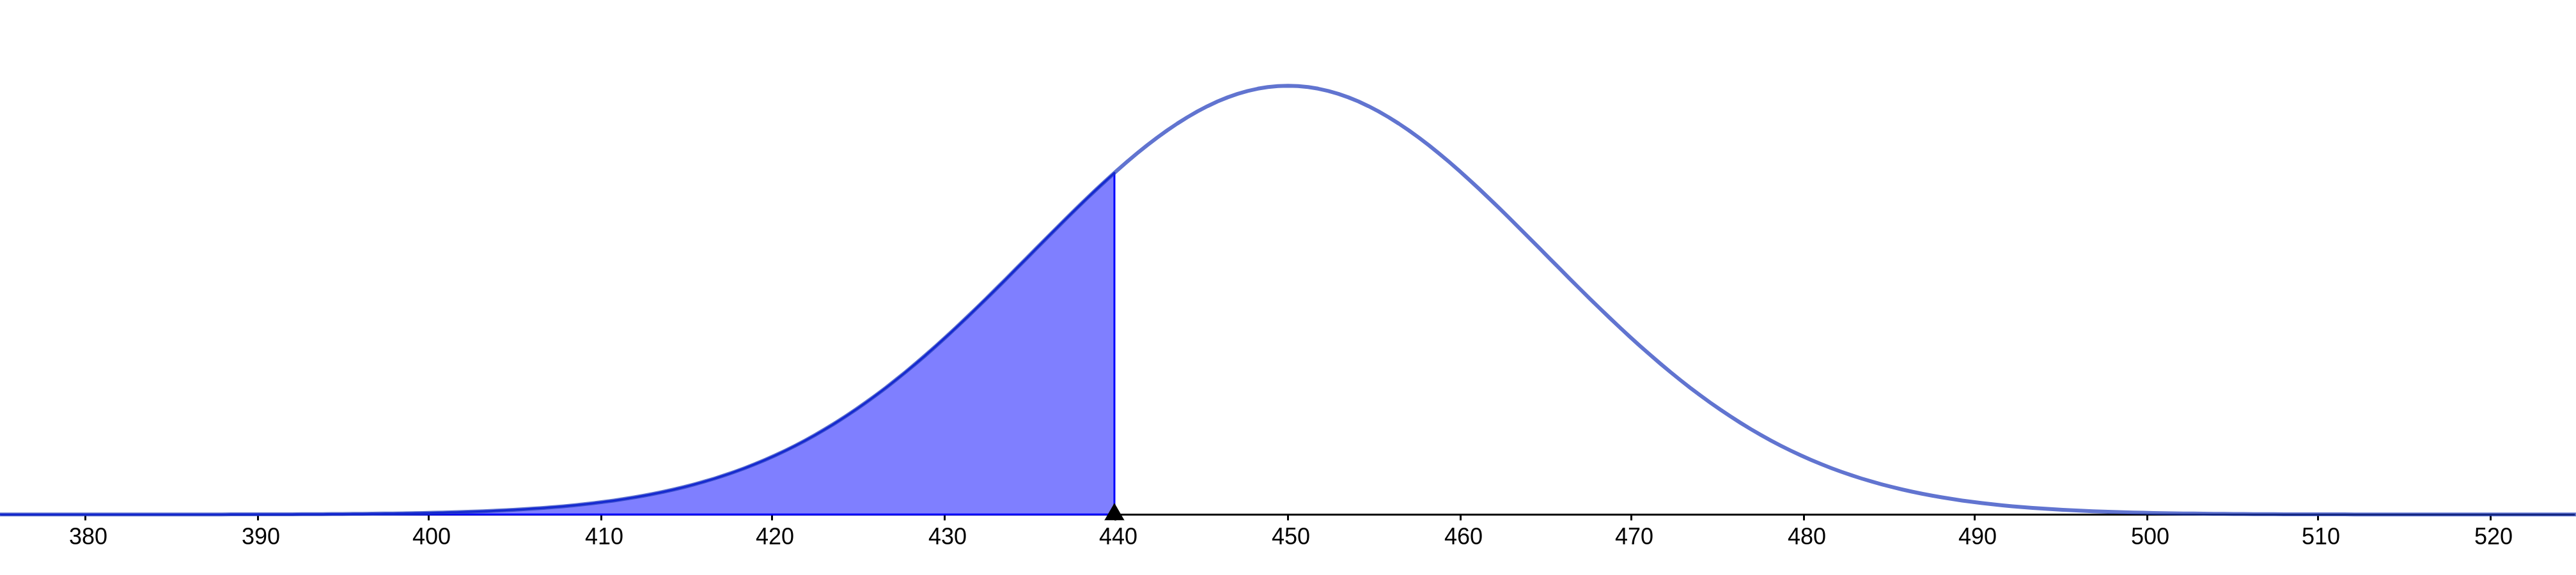
\includegraphics[width=0.6\linewidth]{pics/p2}
			\centering
		\end{figure}
		veremos que el valor es aproximadamente 440 mililitros.
	\end{enumerate}
\end{sol}
\subsection*{Ejercicio 9}[2,5 pts]
	Cierta fabrica manufacturera requiere $f(x)gh(y)$de un producto específico a granel. La cantidad del producto utilizada
	en un día se puede modelar por una $aaa$ distribución exponencial con $\lambda = 4$ (mediciones en toneladas).\textit{A}$A$ Encuentre la
	probabilidad de que la fábrica vaya a utilizar más de cuatro toneladas en un día determinado.

\begin{sol}
	Sea $X$ la cantidad de producto, en toneladas, utilizada en un día. Entonces $X$ es una variable aleatoria con distribución exponencial, cuya función de densidad viene dada por
	\[ 
	f(x) = \begin{cases}
		   \hspace{.2em} \lambda e^{-\lambda x} \quad \text{si} \; x\geq 0 \\
		   \hspace{.5em} 0 \hspace{2.5em} \text{si} \; x<0
		   \end{cases}
	 \]
	 donde, en este caso, $\lambda = 4$.
	 La probabilidad buscada es
	 \begin{align*}
	 	P\{X>4\} &= \int_{4}^{\infty} 4e^{-4x} \mathrm{d}x \\
	 	&= -e^{-4x} \bigg\rvert_{4}^{\infty} \\
	 	&= \frac{1}{e^{16}} \\
	 	&\approx 0.
	 \end{align*}
\end{sol}
\subsection*{Ejercicio 10}
	Suponga que el tiempo, en horas, que toma reparar una bomba es una variable aleatoria $X$ que tiene una
	distribución gamma con parámetros $t = 2$, $\lambda = 1/2$ . ¿Cuál es la probabilidad de que en el servicio siguiente tome cuando mucho una hora reparar la bomba?

\begin{sol}
	Sea $X$ como en el enunciado. Su función de densidad viene dada por
	\[ 
	f(x) = \begin{cases}
	\hspace{.2em} \dfrac{\lambda e^{-\lambda x} (\lambda x)^{t-1}}{\Gamma(t)} \quad \text{si} \; x\geq 0 \\
	\hspace{2.6em} 0 \hspace{3.4em} \text{si} \; x<0
	\end{cases}
	\]
	donde, en este caso, $t=2$ y $\lambda = 1/2$.
	Por propiedades de la función gamma, tenemos que
	\[ \Gamma(2) = (2-1)! = 1. \]
	Ahora la probabilidad buscada es
	\begin{align*}
		P\{X<1\} &= \int_{0}^{1} \frac{1}{2} e^{-x/2} \left(\frac{1}{2} x\right) \mathrm{d}x \\
				 &= \left. -\frac{(x+2)e^{-x/2}}{2} \right\rvert_{0}^{1} \\
			   	 &= -\frac{3e^{-1/2}}{2} + 1 \\
				 &\approx 0.09
	\end{align*}
\end{sol}
\subsection*{Ejercicio 11}
	El tiempo de fallas por fuga de cierto tipo de baterías de celda seca se espera que tenga una distribución
	de Weibull con $a = 0.5$, $\theta = 20$.¿Cuál es la probabilidad de que la batería dure más de 800 horas en uso?

\begin{sol}
	
\end{sol}
\subsection*{Ejercicio 12}
	Si la proporción de televisores de una marca que requiere servicio durante el primer año de operación es
	una variable aleatoria que tiene una distribución beta con $a = 3$, $b = 2$. ¿Cuál es la probabilidad de que al menos
	80\% de los nuevos modelos que se vendan este año requieran servicio durante su primer año de operación? Va Ve

\begin{sol}
	Sea $X$ la proporción de televisores que requieren servicio técnico en el primer año. Entonces $X$ sigue una distribución beta, cuya función de densidad esta dada por
	\[ 
	f(x) = \begin{cases}
	\hspace{.2em} \dfrac{1}{B(a,b)} x^{a-1}(1-x)^{b-1} \quad \text{si} \; 0<x<1 \\
	\hspace{3em} 0 \hspace{6.4em} \text{si} \; x<0
	\end{cases}
	\]
	donde, en este caso, $a = 3$ y $b = 2$.
	
	Veamos primero que
	\[ B(3,2) = \int_{0}^{1} x^2(1-x) \mathrm{d}x = \left. -\dfrac{x^3\left(3x-4\right)}{12} \right\rvert_{0}^{1} = \frac{1}{12}. \]
	La probabilidad buscada es entonces:
	\begin{align*}
		P\left\{X>\frac{4}{5}\right\} &= 12 \int_{4/5}^{1} x^2(1-x) \mathrm{d}x \\
									  &= \left.  -\dfrac{12x^3\left(3x-4\right)}{12} \right\rvert_{4/5}^{1} \\
									  &= 1 - 0.8704 \\
									  &\approx 0.13
	\end{align*}
\end{sol}	
\end{document}